\documentclass{assignment}

\usepackage{float}
\usepackage{tikz}
\usepackage{adjustbox}
\usepackage{titlesec}
\usepackage{soul}
\usepackage{csvsimple}

\usepackage{graphicx}
\usepackage{subcaption}
\usetikzlibrary{shapes, arrows}

\usetikzlibrary{calc,patterns,angles,quotes}
\setlength{\parindent}{0pt}

\hypersetup{
pdftitle={ME663 - Computational Fluid Dynamics},
pdfsubject={Report for assignment 2},
pdfauthor={Tommaso Bocchietti}
}

\makeglossaries

\newacronym{cfd}{CFD}{Computational Fluid Dynamics}
\newacronym{uds}{UDS}{Upwind Differencing Scheme}
\newacronym{cds}{CDS}{Central Differencing Scheme}
\newacronym{hybrid}{HYBRID}{Hybrid Scheme}
\newacronym{quick}{QUICK}{Quadratic Upstream Interpolation for Convective Kinematics}
\newacronym{gs}{GS}{Gauss-Seidel Iterative Method}
\newacronym{scgs}{SCGS}{Symmetric Coupled Gauss-Seidel}
\newacronym{sim}{SIMPLE}{Semi-Implicit Method for Pressure Linked Equations}

\begin{document}

\title{ME663 - Computational Fluid Dynamics \\ Assignment 2}
\author{Tommaso Bocchietti}
\date{A.Y. 2023/24 - W24}

\maketitle

\begin{figure}[H]
    \centering
    
\includegraphics[width=.9\textwidth]{./pdf/UniversityOfWaterloo_logo_vert_pms}
    \label{fig:University_Of_Waterloo_logo}
\end{figure}

\clearpage
\tableofcontents
\listoffigures
\listoftables
\lstlistoflistings
\printglossary[type=\acronymtype]

\clearpage
\section{Introduction}

Every electronic device requires the use of a timing system (usually referred as clock) that sets the reference for the operation of the device.
This timing system is implemented through the use of various electronic components such as clock source, phase comparator, frequency dividers, \dots.

The aim of this project is to investigate the state of the art of clock sources technologies, with a focus on the most recent advancements in the field and their potential applications.
In particular, the project will focus on the following topics:

\begin{itemize}
    \item \semph{Crystal oscillators}: electric oscillator type circuit that uses a piezoelectric resonator, a crystal, as its frequency-determining element (\href{https://en.wikipedia.org/wiki/Crystal_oscillator#Terminology}{Wikipedia definition}).
    \item \semph{\acrshort{mems} resonators}: small electromechanical structures that vibrate at high frequencies (\href{https://en.wikipedia.org/wiki/Microelectromechanical_system_oscillator#Resonators}{Wikipedia definition}).
    \item \semph{\acrshort{mems} Atomic Clocks} (time permitting): the combination of a \acrshort{mems} system fabrication with atomic clocks for small, cheap, low-power devices \cite{KNAPPE2008571}.
\end{itemize}



\section{Methods}
\label{sec:methods}

\paragraph{Research Methodology}
The research will be conducted through a literature review of scientific articles, conference papers and thesis if available.
The main sources of information will be the IEEE Xplore, ScienceDirect, and Google Scholar databases.
The search will be conducted using the following keywords: "Chip-Scale Atomic Clock", "Atomic Clock", "MEMS", "CSAC", "Vapor Cell", "Rubidium", "Cesium", "Microwave Cavity", "Laser Cooling", "Photon Detector", "Quartz Crystal Oscillator", "Electron Spin", "Electron Excitation", "Optical Lattice Clock", "Quantum Technologies".

During the research, we will try to annotate the most relevant papers and articles, that will be then used to write the final report.

\paragraph{Outline}
We leave here a general outline that will be used as a guide for the development of the project.

\begin{enumerate}
    \item Introduction: Discuss the need for precise timekeeping and the exigence of chip-scale atomic clocks.
    \item \textbf{Engineering of Chip-Scale Atomic Clocks}: Discuss the principles of operation. Note: It would be interesting to use simulation tools such as \texttt{COMSOL Multiphysics} to visualize the operating principles of these devices, but not knowing the software and its capabilities, I am not sure if it is applicable here.
          \begin{itemize}
              \item Vapour cell
              \item Magnetic selector (electron spin)
              \item Microwave cavity (electron excitation at hyperfine transition)
              \item Laser system (laser cooling and trapping of atoms)
              \item Photon detector
              \item Closed loop over quartz crystal oscillator
          \end{itemize}
          \begin{figure}[H]
              \centering
              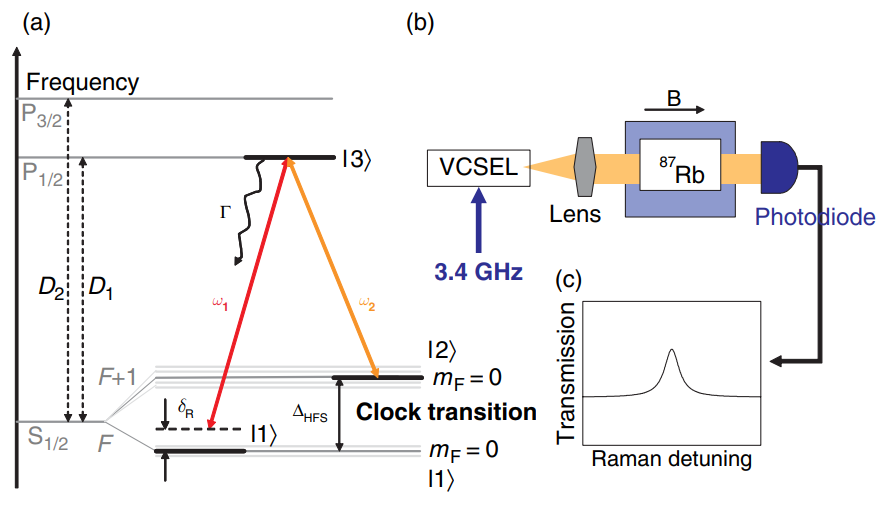
\includegraphics[width=.6\textwidth]{img/atomic_clock_logic}
              \caption{Schematic of the simplified atomic energy level configuration \cite{KNAPPE2008571}}
          \end{figure}

    \item \textbf{Technology Comparison}: Introduce the different types of chip-scale atomic clocks. Compare and contrast the different chip-scale atomic clock technologies in terms of size, power consumption, accuracy, and suitability for various applications.
          \begin{itemize}
              \item Cesium based
              \item Rubidium based
          \end{itemize}
          % \item Fabrication and Manufacturing: Explore the components of chip-scale atomic clocks such as atomic vapor cells, laser systems, and control electronics. Understand the microfabrication techniques used in their manufacturing.
    \item Applications: Consider the diverse applications of chip-scale atomic clocks (aerospace and defense to telecommunications and scientific research)
    \item Challenges and Future Directions: Identify current challenges such as size reduction and power efficiency, and consider future trends like adoption of optical lattice clocks and integration with quantum technologies.
    \item Conclusion: Summarize the key findings of the research and discuss the implications for future advancements and applications of chip-scale atomic clocks.
\end{enumerate}

% In case of time availability, we will also cover the Fabrication and Manufacturing of these devices, understanding the microfabrication techniques used in their manufacturing.

\paragraph{Time schedule}
In general, given a time constraint of 4/5 weeks, the project will be divided as follows (tentative)

\begin{itemize}
    \item Week 1: Introduction + Engineering of Chip-Scale Atomic Clocks
    \item Week 2: Engineering of Chip-Scale Atomic Clocks (possible simulation and results analysis)
    \item Week 3: Technology Comparison + Applications
    \item Week 4: Challenges and Future Directions + Conclusion
    \item Week 5: Final report writing
\end{itemize}

\section{(Q1) - Question \#1}
\label{sec:Q1}

Derive the Jacobian matrix $A = \frac{\partial F}{\partial U}$ given:

\begin{equation}
    U = \begin{bmatrix}
        \rho   \\
        \rho u \\
        \rho E
    \end{bmatrix}, \quad
    F = \begin{bmatrix}
        \rho u       \\
        \rho u^2 + p \\
        (\rho E + p) u
    \end{bmatrix}
\end{equation}

where $\rho$ is the density, $u$ is the velocity, $E$ is the total energy, and $p$ is the pressure.

\subsection{Solution}

The Jacobian matrix $A$ is defined as:

\begin{equation}
    A = \frac{\partial F}{\partial U} = \begin{bmatrix}
        \frac{\partial F_1}{\partial U_1} & \frac{\partial F_1}{\partial U_2} & \frac{\partial F_1}{\partial U_3} \\
        \frac{\partial F_2}{\partial U_1} & \frac{\partial F_2}{\partial U_2} & \frac{\partial F_2}{\partial U_3} \\
        \frac{\partial F_3}{\partial U_1} & \frac{\partial F_3}{\partial U_2} & \frac{\partial F_3}{\partial U_3}
    \end{bmatrix}
    \label{eq:jacobian_matrix}
\end{equation}

where $F_i$ is the $i$-th component of the vector $F$ and $U_i$ is the $i$-th component of the vector $U$.

Before proceeding with the derivation of the Jacobian matrix, it's useful to express the components of the vector $F$ in terms of the components of the vector $U$:

\begin{equation}
    F = \begin{bmatrix}
        \rho u       \\
        \rho u^2 + p \\
        (\rho E + p) u
    \end{bmatrix} = \begin{bmatrix}
        U_2                                                                       \\
        \frac{U_2^2}{U_1} + (\gamma - 1) \left( U_3 - \frac{U_2^2}{2 U_1} \right) \\
        \frac{U_2}{U_1} \left( U_3 + (\gamma - 1) \left( U_3 - \frac{U_2^2}{2 U_1} \right) \right)
    \end{bmatrix}
\end{equation}

Now, we can proceed with the derivation of the Jacobian matrix $A$ based on its definition in Equation \ref{eq:jacobian_matrix}:

\begin{equation}
    A = \frac{\partial F}{\partial U} = \begin{bmatrix}
        0                             & 1                                        & 0          \\
        \frac{\gamma - 3}{2} u^2      & (3 - \gamma) u                           & \gamma - 1 \\
        (\gamma - 1) u^3 - \gamma u E & -\frac{3}{2} (\gamma - 1) u^2 + \gamma E & \gamma u   \\
    \end{bmatrix}
\end{equation}


\section{(Q2) - Question \#2}
\label{sec:Q2}

Derive the right eigenvectors $r_1$, $r_2$, and $r_3$ for the matrix $A$ (Equation \ref{eq:matrix_A}).
Note that:

\begin{equation}
    Q_A = \begin{bmatrix}
        r_1 & r_2 & r_3
    \end{bmatrix}
\end{equation}

\subsection{Solution}

The right eigenvectors $r_1$, $r_2$, and $r_3$ of the matrix $A$ are defined as the eigenvectors that satisfy the following equation:

\begin{equation}
    A Q_A = Q_A \Lambda
\end{equation}

where $\Lambda$ is the diagonal matrix of the eigenvalues of $A$ and $Q_A$ is the matrix of the right eigenvectors of $A$.

To solve the eigenvalues and eigenvectors problem, we can use its characteristic equation:

\begin{equation}
    \text{det}(A - \lambda I) = 0
\end{equation}

where $I$ is the identity matrix.

The characteristic equation for the matrix $A$ is:

\begin{equation}
    \text{det}(A - \lambda I) = \text{det}\left( \begin{bmatrix}
            -\lambda                      & 1                                        & 0                  \\
            \frac{\gamma - 3}{2} u^2      & (3 - \gamma) u - \lambda                 & \gamma - 1         \\
            (\gamma - 1) u^3 - \gamma u E & -\frac{3}{2} (\gamma - 1) u^2 + \gamma E & \gamma u - \lambda
        \end{bmatrix} \right) = 0
\end{equation}

Expanding the determinant, we get:

\begin{equation}
    -\lambda \left[ (3 - \gamma) u - \lambda \right] \left[ \gamma u - \lambda \right] - \frac{\gamma - 3}{2} u^2 \left[ \gamma u - \lambda \right] - (\gamma - 1) \left[ (\gamma - 1) u^3 - \gamma u E \right] = 0
\end{equation}

Solving the characteristic equation, we find the eigenvalues of the matrix $A$:

\begin{equation}
    \Lambda = \begin{bmatrix}
        u & u + c & u - c
    \end{bmatrix}
    \label{eq:matrix_Lambda}
\end{equation}

where $c = \sqrt{\gamma p / \rho}$ is the speed of sound.

The right eigenvectors $r_1$, $r_2$, and $r_3$ of the matrix $A$ are:

\begin{equation}
    r_1 = \begin{bmatrix}
        1 \\
        u \\
        \frac{u^2}{2}
    \end{bmatrix}, \quad
    r_2 = \begin{bmatrix}
        1     \\
        u + c \\
        H + u c
    \end{bmatrix}, \quad
    r_3 = \begin{bmatrix}
        1     \\
        u - c \\
        H - u c
    \end{bmatrix}
    \label{eq:right_eigenvectors}
\end{equation}

where $H = E + p / \rho$ is the enthalpy.

If we rewrite the right eigenvectors in terms of the primitive variables contained in the vector $U$, and adjust the modulus of each eigenvector to match the one of the $Q_A$ reported in \cite{Ghia1982HighReSF}, we get:

\begin{equation}
    Q_A = \begin{bmatrix}
        r_1 & r_2 & r_3
    \end{bmatrix} = \begin{bmatrix}
        1             & \frac{\rho}{2c}                                                & - \frac{\rho}{2c}                                                \\
        u             & \frac{\rho}{2c} (u + c)                                        & - \frac{\rho}{2c} (u - c)                                        \\
        \frac{u^2}{2} & \frac{\rho}{2c} (\frac{u^2}{2} + \frac{c^2}{\gamma - 1} + u c) & - \frac{\rho}{2c} (\frac{u^2}{2} + \frac{c^2}{\gamma - 1} - u c)
    \end{bmatrix}
    \label{eq:matrix_Q_A}
\end{equation}

The code of Mathematica used to derive the right eigenvectors $r_1$, $r_2$, and $r_3$ is reported below:

\lstinputlisting[
    style=mathematica,
    language=Mathematica,
    caption=Mathematica notebook for Q2.,
]{files/Q2.txt}



\section{(Q3) - Question \#3}
\label{sec:Q3}

Derive the following flux-vector splitting:

\begin{equation}
    F^\pm = \left( \frac{\rho}{2\gamma} \right) \begin{bmatrix}
        2(\gamma - 1) \lambda_1^\pm + \lambda_2^\pm + \lambda_3^\pm                  \\
        (2 - \gamma) \lambda_1^\pm u + \lambda_2^\pm (u + a) + \lambda_3^\pm (u - a) \\
        (\gamma - 1) \lambda_1^\pm u^2 + \frac{\lambda_2^\pm}{2} (u + a)^2 + \frac{\lambda_3^\pm}{2} (u - a)^2 + \frac{3-\gamma}{2(\gamma - 1)} (\lambda_2^\pm + \lambda_3^\pm) a^2
    \end{bmatrix}
    \label{eq:flux_vector_splitting}
\end{equation}

Which is equivalent to the following:

\begin{equation}
    F^\pm = \frac{1}{\gamma} Q_A \begin{bmatrix}
        (\gamma - 1) \rho \lambda_1^\pm \\
        a \lambda_2^\pm                 \\
        -a \lambda_3^\pm
    \end{bmatrix}
\end{equation}

Where $Q_A$ is the eigenvector matrix (Equations \ref{eq:matrix_Q_A}).

\subsection{Solution}

We know that the flux-vector $F$ can be expressed as:

\begin{equation}
    F = A U = Q_A \Lambda Q_A^{-1} U
\end{equation}

In order to proof the given flux-vector splitting, we will perform the matrix multiplication given the definitions of the eigenvector matrix $Q_A$ (Equation \ref{eq:matrix_Q_A}) and the diagonal matrix of the eigenvalues $\Lambda$ (Equation \ref{eq:matrix_Lambda}).

The flux-vector splitting can be expressed as follows:

\begin{equation}
    F^\pm = \begin{bmatrix}
        \frac{\rho  (-a+2 \gamma  \lambda_1^\pm-2 \lambda_1^\pm+\lambda_2^\pm+u)}{2 \gamma }                                                                                                        \\
        \frac{\rho  \left(a^2+a (\lambda_2^\pm-2 u)+u (2 (\gamma -1) \lambda_1^\pm+\lambda_2^\pm+u)\right)}{2 \gamma }                                                                              \\
        \frac{\rho  \left(-2 a^3+2 a^2 (\lambda_2^\pm+\gamma  u)-a (\gamma -1) u (3 u-2 \lambda_2^\pm)+(\gamma -1) u^2 (2 (\gamma -1) \lambda_1^\pm+\lambda_2^\pm+u)\right)}{4 (\gamma -1) \gamma } \\
    \end{bmatrix}
\end{equation}

From here, we still can't see the equivalence with the given expression.

We can now compute the coefficients that multiply each $\lambda_i^\pm$.
For simplicity, we will consider the expression $\frac{F^\pm}{\frac{\rho}{2*\gamma}}$, obtaining the following coefficient matrix ($[\text{Known term}, \text{Coef}_{\lambda_1}, \text{Coef}_{\lambda_2}, \text{Coef}_{\lambda_3}]$)

\begin{equation}
    \text{CoefficientList} = \begin{bmatrix}
        u-a                                                   & 2 (\gamma -1)    & 1                                           & 0 \\
        (a-u)^2                                               & 2 (\gamma - 1) u & a+u                                         & 0 \\
        \frac{1}{2} (u-a) (\frac{2 a^2}{\gamma -1}-2 a u+u^2) & (\gamma -1) u^2  & \frac{a^2}{\gamma -1} + a u + \frac{u^2}{2} & 0 \\
    \end{bmatrix}
\end{equation}

From now on, we can carry on the computation of the coefficients by hand, simplifying the coefficient and obtaining the desired result.

\begin{align}
    F^\pm & = \frac{\rho}{2\gamma} \begin{bmatrix}
                                       u-a                                                   & + & 2 (\gamma -1) \lambda_1^\pm    & + & 1    \lambda_2^\pm                                          & + & 0 \lambda_3^\pm \\
                                       (a-u)^2                                               & + & 2 (\gamma - 1) u \lambda_1^\pm & + & a+u  \lambda_2^\pm                                          & + & 0 \lambda_3^\pm \\
                                       \frac{1}{2} (u-a) (\frac{2 a^2}{\gamma -1}-2 a u+u^2) & + & (\gamma -1) u^2 \lambda_1^\pm  & + & (\frac{a^2}{\gamma -1} + a u + \frac{u^2}{2}) \lambda_2^\pm & + & 0 \lambda_3^\pm
                                   \end{bmatrix} =         \\
          & =   \frac{\rho}{2\gamma} \begin{bmatrix}
                                         \lambda_3^\pm + 2 (\gamma -1) \lambda_1^\pm                                                                 + \lambda_2^\pm       \\
                                         \lambda_3^\pm (a+u) + 2 (\gamma - 1) u \lambda_1^\pm                                                        + \lambda_2^\pm (a+u) \\
                                         \frac{\lambda_3^\pm}{2} (u^2 - 2 a u + a^2 + \frac{2 a^2}{\gamma -1} - a^2) + (\gamma -1) u^2 \lambda_1^\pm + \frac{\lambda_2^\pm}{2} (u^2 - 2 a u + a^2 + \frac{2 a^2}{\gamma -1} - a^2)
                                     \end{bmatrix} = \\
          & = \frac{\rho}{2\gamma} \begin{bmatrix}
                                       2 (\gamma -1) \lambda_1^\pm + \lambda_2^\pm + \lambda_3^\pm                   \\
                                       2 (\gamma -1) \lambda_1^\pm u + \lambda_2^\pm (u + a) + \lambda_3^\pm (u - a) \\
                                       (\gamma - 1) \lambda_1^\pm u^2 + \frac{\lambda_2^\pm}{2} (u + a)^2 + \frac{\lambda_3^\pm}{2} (u - a)^2 + \frac{3-\gamma}{2(\gamma - 1)} (\lambda_2^\pm + \lambda_3^\pm) a^2
                                   \end{bmatrix}
    \label{eq:Q3_result}
\end{align}

The result in Equation \ref{eq:Q3_result} is equivalent to the given expression in Equation \ref{eq:flux_vector_splitting}.

The code of Mathematica used to derive the coefficients list:

\lstinputlisting[
    style=mathematica,
    language=Mathematica,
    caption=Mathematica notebook for Q3.,
]{files/Q3.txt}



\section{(Q4) - Question \#4}
\label{sec:Q4}

Following Q3, show that $\lambda^\pm$ in $F^\pm$ corresponding to van Leer's flux-vector splitting method are:

\begin{align}
    \lambda_1^\pm & = \frac{a}{4} (M + 1)^2 \left[1 - \frac{(M - 1)^2}{\gamma + 1}\right]                                   \\
    \lambda_2^\pm & = \frac{a}{4} (M + 1)^2 \left[3 - M + \frac{\gamma - 1}{\gamma + 1} (M - 1)^2\right]                    \\
    \lambda_3^\pm & = \frac{a}{4} (M + 1)^2 \left(2 \frac{M - 1}{\gamma + 1}\right) \left[1 + \frac{\gamma - 1}{2} M\right]
\end{align}

\section{(Q5) - Question \#5}
\label{sec:Q5}

Write a computer code for Test Case 1 (Handout \#4, p. 352) using both Steger-Warming and van Leer flux-vector splitting methods, and compare your numerical results with the exact solutions at $t = 0.01 $for $-10 \le x \le 10$ in terms of density, velocity, pressure, Mach number.

\clearpage
\bibliographystyle{plain}
\bibliography{references}

\clearpage
\appendix
\label{sec:appendix}

\section{Mathematica code}

Here follows the \texttt{Mathematica} notebook used for symbolic analysis of the discretized schemes.

% \lstinputlisting[
%     style=mathematica,
%     language=Mathematica,
%     caption=Mathematica notebook used for symbolic analysis of the discretized schemes.,
% ]{files/Mathematica.txt}

\end{document}
